\documentclass[11pt]{article} % 11pt article, want AMS fonts.

\usepackage{amsmath,amsfonts,amssymb}
\usepackage{latexsym}
\usepackage{hyperref}
\usepackage{graphicx}
\graphicspath{ {./images/} }
\usepackage{setspace}
\usepackage{blindtext}
\usepackage[a4paper, total={6in, 8in}]{geometry}
\usepackage[demo]{graphicx}
\usepackage{subfig}
\usepackage{indentfirst}
\usepackage{changepage}
\usepackage{booktabs}
\usepackage{array}
\usepackage{mathtools}
% \singlespacing
% \onehalfspacing
\spacing{1.1} %to change spacing if necessary 


\begin{document}

\title{How Much Is A Best Picture Oscar Worth?}
\author{Isabella Cha, Kevin Phung, Aryan Arora}
\maketitle

\section{Introduction}
The Academy of Motion Picture Arts and Sciences granted the first Oscars in 1929, creating what is today the oldest, most visible, and most prestigious award in the film industry (Levy 2001). The Academy Awards, now officially the Oscars, has changed little since 1929---the nominees and winners are still decided by the members of the Academy, the nominees are revealed a month or two before the awards ceremony, and the winners are announced at the ceremony.

The existing literature suggests that movies are “experience goods”, defined as “products which consumers choose, buy and use solely to experience and enjoy” (Sawhney and Eliashberg 1996). The intangible and experiential nature of movie consumption makes it difficult to judge movie quality before it is actually viewed; as such, consumers may seek other signals prior to the consumption experience (Bristor 1990; Harrison-Walker 2001; Y. Liu 2006). The Oscars, arguably the most important award in the movie industry, is thought to be an important signal in shaping consumer perceptions (Ginsburgh 2003). The movies that receive this honor go down in history as films of quality and prestige. As noted by Levy (2001), “No other award so well combines critical and popular judgment”. Through the Oscars, the Academy functions as peers, critics, and tastemakers — thus, the question of \textit{how much} an Oscar is worth is a pertinent one. 

In this paper, we are particularly concerned with the ‘Best Picture’ award, the highest honor of the ceremony. We define “worth” as commercial success, as measured by box office revenues. We will use econometric tools to measure whether winning a Best Picture Oscar increases consumers’ demand for a movie by significantly increasing weekly box office revenues. Our results show that Best Picture nominations boost movies’ revenues, whereas the effect of a win is not significant.  



\section{Theoretical Framework}
A movie’s box office revenue is directly related to the number of consumers purchasing tickets to view the movie. Economic theory suggests that the number of tickets sold is a function of consumer demand for seeing a given movie. Factors affecting consumer’s demand are likely to include the number of theaters, theater run, budget, genre, rating, whether the movie features a “star”, and/or released around a holiday. 

\subsection{Possible Determinants of Movie Demand} 
\setlength\parindent{0pt}

\begin{adjustwidth}{1cm}{}

\textbf{Number of theaters} \newline
A greater number of theaters implies a higher probability that consumers have easier access to see a given movie; if a moviegoer is deciding between different movies, all else equal, then they are more likely to see the one screening closest to them. Some consumers may not decide what to watch until entering the theater, all else equal, the likelihood of watching a movie would increase with the movie being shown in more theaters. If no theaters were showing the movie, then ticket sales would effectively be zero. \\


\textbf{Budget}\newline
Higher budget could allow for more spending on factors that could improve movie quality, such as better camera equipment, higher quality editing, and better sound. In addition, a higher budget allows for more spending on advertising and promotion which would also increase demand. Previous studies suggest that high budget films generate more revenues (Deuchert et. al 2005), albeit with varying degrees of elasticity.  
\\

\textbf{Genre}\newline
Film genres appeal differentially to moviegoers. For example, animated and family films are the most popular genre for children accompanied by parents, action/adventure films appeal to younger audiences, and dramas are more popular among older audiences (Redondd and Holbrook 2010). A movie’s strongest competition comes from other movies that are most alike in genre (Elberse 2005; Y. Liu 2006). From this, we postulate that movies in the same genre category may be substitutes; all else equal, a bigger number of substitutes would decrease quantity demanded. 
 \\

\textbf{MPAA Rating}\newline
The MPAA rating of movies may attract or repel certain audiences. G and PG rated movies may be more appealing to families, whereas R-rated movies may appeal to more mature audiences. However, the effect of MPAA ratings may be ambiguous: for instance, the presence of obscene language, explicit sex, and/or violence was reported as the second most important factor in avoiding R-rated movies (Moon et al. 2010) for R-rated movies. On the other hand, some studies suggest sexual content is intrinsically profitable precisely \textit{because} of its controversial nature (Pennington 2007). \\

\textbf{Holiday}\newline
Whether or not a movie was released around a holiday may be a determinant of movie demand. The number of moviegoers varies dramatically throughout the year according to Einav (2007), who observes a “seasonal pattern” of movie sales, with the biggest hits in the beginning of the Christmas holiday season. However, it is also plausible that consumers may prefer to stay at home with family rather than go to movie theaters on Christmas. \\

\textbf{Star Power}\newline
Star power is considered to be one of the key drivers of motion picture success, albeit with some controversy. As Bill Mechanic, former chairman of Twentieth Century Fox put it, “a guy stranded on an island without Tom Hanks is not a movie… there's no way to replace that kind of star power.”  Elberse (2007) finds that on the basis of a multiple regression model, star power has no significant box office sales. On the other hand, Prag and Casavant (1994) found that star power and winning an Academy Award are “unambiguous positive factors in a movie’s financial success.” 
\end{adjustwidth}


\setlength{\parindent}{20pt}

\section{Data}
\subsection{Data Collection} 
Our dataset includes all Oscar-Best picture nomianted movies that were released in the US after January 1, 2000, and which official domestic (US) running time did not exceed December 31, 2019. In order to isolate the effect of the Oscar event, we exclude films that were not nominated. We also decided to exclude movies running from 2020 and beyond due to the COVID-19 pandemic and the shutdown of theaters. We then collected data for our dependent variable and possible explanatory variables as outlined in our theoretical framework. 

Weekly box office returns, and release dates are taken from boxofficemojo.com. To check whether awards influence success, we look at weekly revenue (as opposed to gross revenues) to account for the income generated after the Oscars announcement, in order to be able to determine whether it is the Oscar announcement that triggered the additional income. It is also important to note that the industry operates on a weekly schedule --— much of the competition is over the weekend audience. Consequently, release dates are tabulated at the weekly level. Budget data was taken from the-numbers.com. As the budget data was inflation adjusted, we also used a CPI calculator online with 2000 as the base year, and adjusted all our box office returns for inflation.

Nominations, wins, details on genre, movie content ratings were taken from Internet Movie Database (IMDb). Additionally, data for movie budgets was scraped from The-Numbers (https://www.the-numbers.com/). Star power was constructed from Forbes, List of 100 Highest paid Actors and Actresses for each respective year. 

As final step, we merged and cleaned our datasets from various website using automated Python scripts. Our final dataset includes 125 movies and weekly revenue data for each movie. In total, we have 2999 observations. 


\subsection{Description of Variables}

%Dep var %
\begin{table}[h]
\caption{Dependent Variable}
\label{tab:my-table}
\resizebox{\textwidth}{!}{%
\begin{tabular}{|l|l|}
\hline
\textbf{Variable Name} &
  \textbf{Description} \\ \hline
\textit{WeeklyEarning} &
  \begin{tabular}[c]{@{}l@{}}Revenues from US ticket sales, measured in USD. \\ Does not include DVD rentals, streaming purchases, or additional releases of the film.\end{tabular} \\ \hline
\end{tabular}%
}
\end{table}

% EXP VARS
\begin{table}[h]
\caption{Possible Explanatory Variables}
\label{tab:my-table}
\resizebox{\textwidth}{!}{%
\begin{tabular}{|l|l|}
\hline
\textbf{Variable Name}    & \textbf{Description}                                                   \\ \hline
\textit{Cumulative Weeks} & Number of weeks after release, starting from 1.                        \\ \hline
\textit{Cumulative Gross} & Gross revenues up till the point of nomination                        \\ \hline

\textit{Weekly rank}      & Rank of the movie relative to other movies in terms of revenue.        \\ \hline
\textit{Theaters}         & Number of cinema cites showing the movie. Only includes US theaters.   \\ \hline
\textit{Budget}           & Movie production budget, measured in USD.                              \\ \hline
\textit{MPAA Rating (3 categories)}      & \begin{tabular}[c]{@{}l@{}}(1) PG\\ (2) PG-13\\ (3) R\end{tabular}     \\ \hline\textit{Genre (5 groupings)} &
  \begin{tabular}[c]{@{}l@{}}6 different genre groupings: \\ (1) Action, Adventure, Fantasy, Sci-Fi (AAFS); \\ (2) Drama,Comedy,Romance (DCR); \\ (3) Crime, Mystery, Horror, Thriller (CMHT); \\ (4) Biography, Sport, History, War (BSHW); \\ (5) Animation, musical, family (AMF); \\ Each genre grouping is a dummy variable, \\which takes on a value of 1 if the movie is classified as part of the grouping.\\
  In order to account for the dummy variable trap, we removed one category (Western) \\ that was deemed multicollinear. 
                       \\ \hline
  
  \end{tabular} \\ \hline
\textit{Holiday (Constructed)} &
  \begin{tabular}[c]{@{}l@{}} A binary variable to indicate if a movie is released in the holiday season.\\ "Holiday season" is defined as: the last 6 weeks of the calendar year.\end{tabular} \\ \hline
\textit{Star power (Constructed)} &
  \begin{tabular}[c]{@{}l@{}}A binary variable to indicate if the movie has star power. \\ A movie is classified as having star power if:\\ at least one of its main cast members appears in the Forbes list of 100 top-paid actors and \\actresses in their respective year of release. \\ This classification is in similar fashion with previous studies done on star power \\(Liu Y. 2006; Liu, A. et. al 2014).\end{tabular} \\ \hline
\textit{Oscar Nomination} & A binary variable if a movie was nominated for the Best Picture Oscar. \\ \hline
\textit{Oscar Win}        & A binary variable if a movie won the Best Picture Oscar.               \\ \hline
\end{tabular}%
}
\end{table}
\footnote{In the Correlation Table we refer to the number of theaters variable as 'Num\_T' in order to fit all names, everywhere else it is referred to as 'num\_theater'}

\newpage


\subsection{Exploratory Data Analysis}

Prior to drawing up our model, we created a heatmap of a correlation matrix in an attempt to detect high levels of correlation between our explanatory variables. We found the highest to be 0.68, which was not high enough to cause any problems for us.

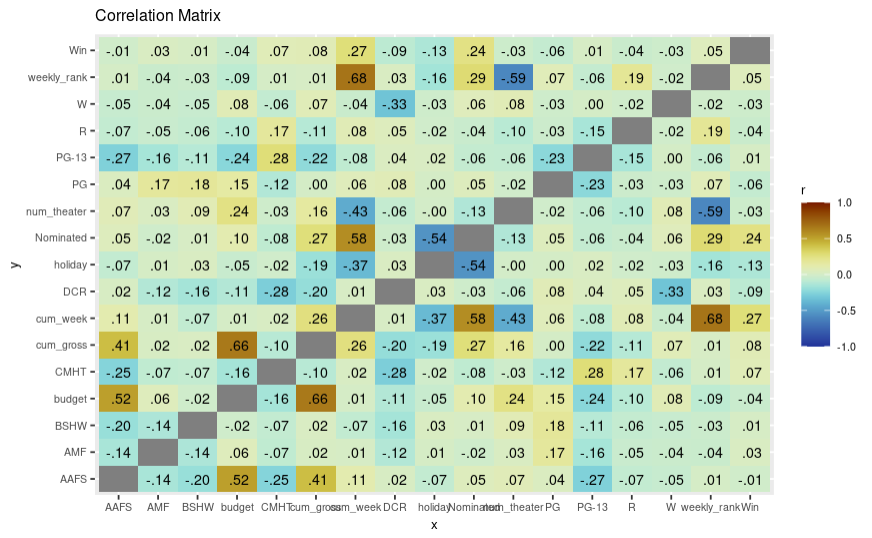
\includegraphics[scale=0.85]{version2/heatmap.png}

\section{Model Specification}


Given our economic theory for the variables we considered, we began by creating a model with all of our variables. We then ran F and T tests on the variables for which we did not have a strong enough economic theory and thus wanted to examine. We first ran an F test on both Genre and Ratings. This approach is a product of two considerations. The first is the risk of the ommited variable bias, the second is a comparatively larger risk of underfitting as compared to overfitting. Given the size of our dataset (roughly 3000 datapoints) we saw a much larger risk of underfitting and biasing our estimated (as shown by the ommited variable bias) as compared to overfitting. Thus we tried to include as many theoretically sensible variables as we could think of an run tests on those we did not have substantial economic theory to decide one way or another (namely ratings, genre, star power, and an interaction between win and cumulative earnings). 

Our F test on Genre produced a statistically significant result at a 5\% significance level (p value = 0.0009393). This meant that the restriction (removing the genre dummy variables) significantly worsened the goodness of fit. 

Our F test on Rating did not produce a statistically significant result at a 5\% significance level (p value = 0.09054). This meant that the restriction (removing the rating dummy variables) did not significantly worsen the goodness of fit. 

Furthermore the T test on the star power explanatory variable did not provide a statistically significant result at a 1\% level of significance (p value = 0.03873). Given that we did not have sufficient economic theory justifying star power as a predictor of film earnings, we held a high threshold to include it in the model (hence 1\%), and thus we decided to omit the variable. We also removed the interaction between cumulative gross earnings and and win for similar reasons (p value = 0.88290).

Additionally, we then conducted tests for linearity and found non-linearity. We also ran a Ramsey Reset Test for a quadratic model. Our Reset statistic (RESET = 75.65, df1 = 12, df2 = 2972) provided evidence against the linear model, but we were inconclusive on the structure of the correct model. We resolved the non-linearity by logging the dependent variable: weekly earnings. This provided the following Histogram and QQ plot: 

\begin{figure} [h]
    \centering
    \subfloat{{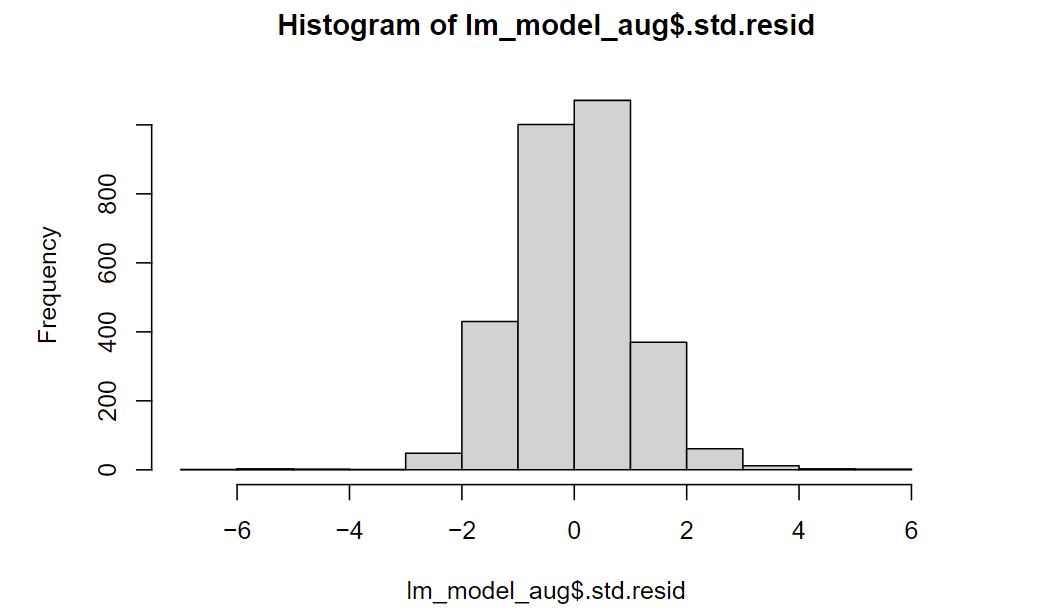
\includegraphics[scale = 0.3]{version2/residual_histo.png} }}%
    \qquad
    \subfloat{{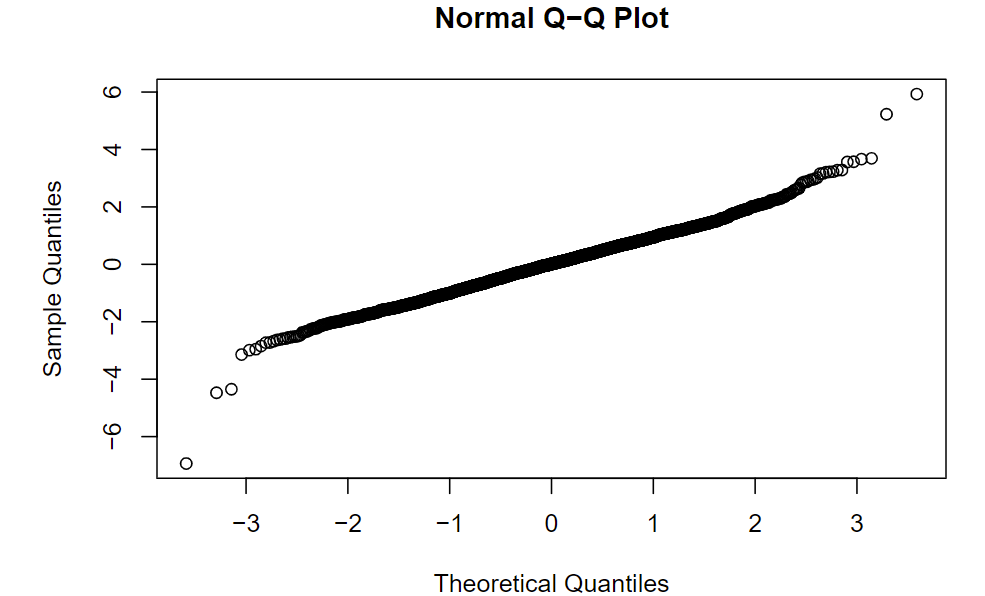
\includegraphics[scale = 0.3]{version2/QQ_plot.png}}}%
    \label{fig:example}%
\end{figure}

We did not conduct a Shapiro-Wilk test, as the test is highly sensitive when we have a large sample size. At large sample sizes, the probability of rejecting the null hypothesis that the residuals are normally distributed becomes extremely large, leading to everything short of perfect normality being rejected by the test. 

Our Breusch-Pagan test for heteroskedascity produced a chi-square statistic that provided strong evidence of heteroskedasticity in our model (BP = 167.5, df = 14). Additionally, our Durbin-Watson statistic (1.177) provided strong evidence for autocorrelation. Because of this, we use Newey-West standard errors in our model that are robust against both heteroskedascity and autocorrelation. 

Given that our exploratory data analysis (the correlation matrix) provided little evidence of multicollinearity, we were satisfied with concluding that there were no pairwise variables that had concerning levels of multicollinearity.

This produces our final model: 
\begin{table}[!htbp] \centering 
\small
  \caption{Final Regression Summary} 
  \label{} 
\begin{tabular}{@{\extracolsep{5pt}}lc} 
\\[-1.8ex]\hline 
\hline \\[-1.8ex] 
 & \multicolumn{1}{c}{\textit{Dependent variable:}} \\ 
\cline{2-2} 
\\[-1.8ex] & Coefficients (Robust Standard Errors(HAC SE)) \\ 
\hline \\[-1.8ex] 
 Nominated & 1.556$^{***}$ \\ 
  & (0.283) \\ 
  & \\ 
 log\_cum\_gross & 0.088$^{***}$ \\ 
  & (0.011) \\ 
  & \\ 
 cum\_week & $-$0.054$^{***}$ \\ 
  & (0.003) \\ 
  & \\ 
 weekly\_rank & $-$0.069$^{***}$ \\ 
  & (0.001) \\ 
  & \\ 
 num\_theater & 0.001$^{***}$ \\ 
  & (0.00001) \\ 
  & \\ 
 Win & $-$0.117$^{***}$ \\ 
  & (0.039) \\ 
  & \\ 
 AAFS & 0.122$^{***}$ \\ 
  & (0.029) \\ 
  & \\ 
 DCR & 0.103$^{***}$ \\ 
  & (0.031) \\ 
  & \\ 
 CMHT & 0.044$^{*}$ \\ 
  & (0.024) \\ 
  & \\ 
 BSHW & $-$0.113$^{***}$ \\ 
  & (0.027) \\ 
  & \\ 
 AMF & 0.096$^{***}$ \\ 
  & (0.034) \\ 
  & \\ 
 log\_budget & $-$0.040$^{***}$ \\ 
  & (0.011) \\ 
  & \\ 
 Nominated:log\_cum\_gross & $-$0.112$^{***}$ \\ 
  & (0.016) \\ 
  & \\ 
 Nominated:cum\_week & 0.035$^{***}$ \\ 
  & (0.003) \\ 
  & \\ 
 Constant & 14.652$^{***}$ \\ 
  & (0.201) \\ 
  & \\ 
\hline \\[-1.8ex] 
Observations & 2,999 \\ 
R$^{2}$ & 0.950 \\ 
Adjusted R$^{2}$ & 0.950 \\ 
Residual Std. Error & 0.483 (df = 2984) \\ 
F Statistic & 4,066.637$^{***}$ (df = 14; 2984) \\ 
\hline 
\hline \\[-1.8ex] 
\textit{Note:}  & \multicolumn{1}{r}{$^{*}$p$<$0.1; $^{**}$p$<$0.05; $^{***}$p$<$0.01} \\ 
\end{tabular} 
\end{table} 
\newpage

\section{Empirical Results and Analysis}

Our goal is to estimate the degree to which the explanatory variables discussed in earlier sections are correlated with the weekly box-office revenues in our sample. To do so, we estimate a standard weekly revenue function of the form: 

\begin{align*}
\mathrm{log(WeeklyEarnings)} = \beta_{0}
    &+ \beta_{1}  \mathrm{Nominated} \\
    &+ \beta_{2}  \mathrm{log(cum\_gross)} \\
    &+ \beta_{3}  \mathrm{cum\_week} \\
    &+ \beta_{4}  \mathrm{weekly\_rank} \\
    &+ \beta_{5}  \mathrm{num\_theater} \\
    &+ \beta_{6}  \mathrm{Win}  \\
    &+ \beta_{7}  \mathrm{AAFS} \\
    &+ \beta_{8}  \mathrm{DCR} \\
    &+ \beta_{9}  \mathrm{CMHT} \\
    &+ \beta_{10}  \mathrm{BSHW} \\
    &+ \beta_{11}  \mathrm{AMF} \\
    &+ \beta_{12}  \mathrm{log(budget)} \\
    &+ \beta_{13}  \mathrm{Nominated*log(cum\_gross)} \\
    &+ \beta_{13}  \mathrm{Nominated*cum\_week} + \epsilon\\
\end{align*}

The explanatory variables are defined as listed in Table 1. 

\subsection{Interpretation of Beta Coefficients}

There is little meaning to an intercept coefficient in a case like ours but the best interpretation we can provide is that a movie, in its first week of production, meaning that it has not been nominated for best picture, has no cumulative gross earnings, has number a cumulative number of weeks of 0, has not been ranked, and is of the AAFS genre, is predicted to earn $e^{14.65}$ or $\$2,303,637.60$ on average.

Based on our model results, holding everything else equal, \textit{Nomination} will lead to a predicted increase in the median weekly revenue of a movie by a multiplicative factor of $e^{1.56}$ or $4.759$. Basically, median weekly revenue is predicted to be \$4.759 times higher if a movie has a nomination than without. 

Holding everything else equal, a 10\% increase in \textit{cumulative\_gross\_earnings} will lead to a predicted increase in the median weekly revenue of a movie by $e^{0.088}$ $0.842\%$.  Basically, median weekly revenue is predicted to be on average \$0.842\% higher if a movie has cumulative gross earnings higher by 10\%.


Holding everything else equal, a 1 week increase in \textit{cumulative\_week} will lead to a predicted decrease in the median weekly revenue of a movie by $e^{-0.054}$ or $-5.26\%$.  Basically, median weekly revenue is predicted to be \$5.26\% lower on average if a movie has been out for an additional week.

Holding everything else equal, a 1 position increase in \textit{weekly\_rank} will lead to a predicted decrease in the median weekly revenue of a movie by $e^{-0.069}$ or $-6.67\%$.  Basically, median weekly revenue is predicted to be on average \$6.67\% lower if a movie drops its movie rank by 1 place.

Holding everything else equal, an increase in\textit{Num\_theater} will lead to an increase in the predicted median weekly revenue of a movie by $e^{-0.00067}$ or $0.06\%$.  Basically, median weekly revenue is predicted to be on average \$0.06\% higher if a movie shows in 1 extra theater.

Holding everything else equal, a win is predicted to decrease the median weekly revenue of a movie by $e^{-0.120}$ or $-11.31\%$. Basically, median weekly revenue is predicted to be on average \$-11.31\% lower if a movie wins the Oscars.

\vspace{\baselineskip} 

For the interpretations of the genres, we will use a Nominated Western movie as the baseline interpretation (for brevity we use the acronyms for our category labels, see section 3.2 for descriptions).

Holding everything else equal, a film of the AAFS genre is predicted to increase the median weekly revenue of a movie by $e^{0.12}$ or $12.7\%$. Basically, median weekly revenue is predicted to be on average \$12.7\% higher if a movie is DCR as compared to W.

Holding everything else equal, a film of the DCR genre is predicted to increase the median weekly revenue of a movie by $e^{0.10}$ or $10.5\%$. Basically, median weekly revenue is predicted to be on average \$10.5\% higher if a movie is DCR as compared to W.

Holding everything else equal, a film of the CMHT genre is predicted to increase the median weekly revenue of a movie by $e^{0.04}$ or $4.08\%$. Basically, median weekly revenue is predicted to be on average \$4.08\% higher if a movie is CMHT as compared to W. As this coefficient was statistically insignificant, it had no effect on our model.

Holding everything else equal, a film of the BSHW genre is predicted to decrease the median weekly revenue of a movie by an effect of $e^{-0.11}$ or $-10.41\%$. Basically, median weekly revenue is predicted to be on average \$10.41\% lower if a movie is W as compared to W.

Holding everything else equal, a film of the AMF genre is predicted to increase the median weekly revenue of a movie by $e^{0.09}$ or $9.42\%$. Basically, median weekly revenue is predicted to be on average \$9.42\% higher if a movie is AMF as compared to W.




\subsection{Analysis}

Our results indicate that Oscar \textit{nominations} have a positive effect, but a win is less statistically significant than nomination, and in fact, is negative. A possible explanation for why a Oscar win is negative may be because of omitted variable bias -- nominated films are in theaters for some time before the Oscars announcement, so they have already built up a certain economic impact. There is a slight "boost" from the nomination, but the win does not change much. Additionally, we suspect that most demand comes from the nomination announcement, where die-hard movie-fans will rush to watch all nominated movies. Thus, demand would have significantly dried up by the time the Oscar awards winner for best picture is announced.

A surprising result was a negative correlation for budget. We think that the negative correlation for budget could be attributed to a form of omitted variable bias, in the sense that we could not split up total movie budget into its component parts, namely advertising, costs of actors, etc. each of which would have very different effects on earnings.

As for genres, the effects seem in-line with expectations in that biographic movies and the-like tend to underperform in the box-office due to their limited appeal to a wider audience.

Lastly, the fact that the estimated coefficient for nomination was positive but the estimated coefficient for the interaction between nomination and log(cumulative\_earnings) was negative was interesting. In particular, we propose that the nomination's effect on a movie is affected by its total earnings so far, with higher total earnings leading to smaller (and in this case negative) gains to the movie's weekly revenue. This makes sense, given that most popular movies that get nominated already have been viewed by most people, and thus do not get any boost from the nomination or win.



\subsection{Limitations}
Our dataset also includes notable outliers such as \textit{Avatar}. For such blockbuster films, it is difficult to say whether awards influence success or whether the Academy goes with the flow or the Oscar win boosted revenues. \textit{Avatar}, for example, made 140 million USD in the first week alone. Due to complications in defining an exact threshold for excluding movies, however, we did not remove these observations — which may have skewed our results towards higher earnings. 


Further, we were working with time-series data but did not have the ability to use time series models, which limited the set of tools for model building to multi-variable regression analysis. For further study, we could use a LSTM model that could better work with time-series data. 

The Ramsey Reset Test provides clear evidence that our model has room for improvement. With stronger economic training and theory as well as further statistical tools we could begin to create a model which had a structure that better fits the data: our Reset test suggested that our linear model does not do that.

\section{Conclusion}


Although our measure of a movie’s ‘success’ is weekly box office revenues, it is also important to acknowledge that the Academy does not blindly endorse the masses, given the Academy’s own proclamation that “excellence in filmmaking is the only factor [to] consider in casting votes” (National Academy, 2022). The votes are cast by, namely, members of the Academy who comprise of “gifted and skilled artists and craftsmen in the motion picture world” -- 8,100 members as of 2019). The panel of judges are chosen on an invite-only basis; the exact criterion is not known to the public. As such, commercial success and Oscar wins may only be associated to the extent that these supposed experts and moviegoers share the same taste. 

Moreover, the movie industry has undergone structural changes during the time frame 2000-2019 for which we collected our data. With the rise of Netflix and other streaming services, box office numbers measuring ticket sales are incomplete and don't show the full picture for the demand of a movie. Nowadays, consumers can enjoy a newly released movie in the comfort of their homes. For a more comprehensive analysis in future studies, we could look at user data from streaming services. 






\newpage
\section*{References}
\leftskip 0.3in
\parindent -0.3in

\noindent 
 
  Bristor, Julia (1990), "Enhanced Explanation of Word of Mouth Communications: The Power of Relationships," in Research in Consumer Behavior, E.C. Hirschman, ed. Greenwich, CT: JAI Press, 51-8

Deuchert,, E., Adjmah, K., & Pauly, F. (2005). For Oscar Glory or Oscar Money? Journal of Cultural Economics, 29(3), 159–176. http://www.jstor.org/stable/41810887 

Elberse, A. (2007). The Power of Stars: Do Star Actors Drive the Success of Movies? Journal of Marketing, 71(4), 102–120. http://www.jstor.org/stable/30164000 

Einav, L. (2007). Seasonality in the U.S. Motion Picture Industry. The RAND Journal of Economics, 38(1), 127–145. http://www.jstor.org/stable/25046296 
 
Ginsburgh, V. (2003). Awards, Success and Aesthetic Quality in the Arts. The Journal of Economic Perspectives, 17(2), 99–111. http://www.jstor.org/stable/3216859 

Harrison-Walker, L. Jean (2001), "The Measurement of Word-of- Mouth Communication and an Investigation of Service Quality and Customer Commitment as Potential Antecedents," Journal of Services Marketing. 

Levy E. (2001) Oscar Fever: The History and Politics of the Academy Awards (The Continuum International Publishing Group, New York). 

Liu, Yong (2006), "Word of Mouth for Movies: Its Dynamics and Impact on Box Office Revenue," Journal of Marketing, 70 (July), 74-89

Liu, A., Liu, Y., & Mazumdar, T. (2014). Star power in the eye of the beholder: A study of the influence of stars in the movie industry. Marketing Letters, 25(4), 385–396. http://www.jstor.org/stable/24571121

Moon, S., Bergey, P. K., & Iacobucci, D. (2010). Dynamic Effects among Movie Ratings, Movie Revenues, and Viewer Satisfaction. Journal of Marketing, 74(1), 108–121. http://www.jstor.org/stable/20619083 

  Pennington, J. W. (2007). The history of sex in American film. Westport: Praeger.

Prag, J. and Casavant, J. (1994). An Empirical Study of the Determinants of Revenues and Marketing Expenditures in the Motion Picture Industry. Journal of Cultural Economics, 18(3), 217–235. http://www.jstor.org/stable/41804889 

Redondo, Ignacio, and Morris B. Holbrook. “Modeling the Appeal of Movie Features to Demographic Segments of Theatrical Demand.” Journal of Cultural Economics 34, no. 4 (2010): 299–315. http://www.jstor.org/stable/41811062.
 
Sawhney, M. S., & Eliashberg, J. (1996). A Parsimonious Model for Forecasting Gross Box-Office Revenues of Motion Pictures. Marketing Science, 15(2), 113–131.\\ http://www.jstor.org/stable/184189




\end{document}
